\documentclass[11pt]{article}

\usepackage[margin=1.0in]{geometry}
\usepackage{amsmath,amsthm,amssymb}
\usepackage{mathtools}
\usepackage{graphicx}
\usepackage{xcolor}
\usepackage{setspace}
\usepackage{multirow}
\usepackage{booktabs}
\usepackage{comment}
\usepackage{dsfont}
\usepackage{authblk}
\usepackage{lineno}
\usepackage{url}
\usepackage{appendix}
\usepackage{natbib}

\bibpunct{(}{)}{;}{a}{}{,}

\definecolor{NAU-Blue}{RGB}{0,51,102}        % NAU True Blue
\definecolor{NAU-Gold}{RGB}{241,179,0}       % NAU Gold

\definecolor{magenta-dark}{RGB}{140,0,140}   % High contrast
\definecolor{magenta-medium}{RGB}{200,0,200}
\definecolor{magenta-light}{RGB}{255,0,255}

\def\T{{\mathrm{\scriptscriptstyle T}}}
\def\spacingset#1{\renewcommand{\baselinestretch}{#1}\small\normalsize}

%\linenumbers
\spacingset{1.1}

\renewcommand*{\Authsep}{, }
\renewcommand*{\Authand}{\authorcr}   % \renewcommand*{\Authand}{, }
\renewcommand*{\Authands}{, }
\renewcommand*{\Affilfont}{\small\normalfont}

%\setlength{\authorsep}{2em}
\setlength{\affilsep}{1.6em}            % set the space between author and affiliation
\setlength{\bibsep}{3pt}


\title{\textbf{Time Series Analysis of Transit Ridership}\vspace{5pt}}

\author[1]{Rylan Harris}
\author[1]{Nick Larson}
\author[1,2]{Eli Vatsaas}

\affil[1]{Department of Mathematics and Statistics, Northern Arizona University, Flagstaff, AZ 86011, USA}

\date{\today}

%------------------------------------------------------------------------------%
\begin{document}
%------------------------------------------------------------------------------%

\maketitle

\begin{abstract}
This study applies time series analysis techniques to investigate patterns in public transit ridership in the United States, with particular attention to the impact of COVID-19. Using monthly Unlinked Passenger Trips (UPT) data from the National Transit Database spanning January 2002 to February 2025, we develop multiple time series models using both manual and automated approaches at national and jurisdictional levels. Our methodology includes fitting SARIMA models to pre-COVID data to estimate counterfactual ridership levels and developing intervention models to capture the structural break caused by the pandemic. Results indicate that while transit ridership follows consistent seasonal patterns, COVID-19 caused unprecedented disruption to ridership levels. Although recovery has occurred, current ridership remains significantly below pre-pandemic forecasted levels, with the recovery rate showing signs of deceleration. The jurisdictional analysis reveals geographical variations in both pre-pandemic patterns and post-pandemic recovery trajectories. This analysis provides valuable insights for transit agencies and policymakers in understanding ridership patterns and the long-term implications of major disruptions on public transportation systems.
\end{abstract}

\vspace{8pt}
\noindent
\textbf{Keywords}: Time series analysis; SARIMA models; Public transportation; COVID-19 impact; Ridership forecasting; Intervention analysis.

%------------------------------------------------------------------------------%
\section{Introduction}
%------------------------------------------------------------------------------%

Public transit systems represent critical infrastructure in urban environments, supporting economic activity, reducing traffic congestion, and providing essential mobility for millions of Americans. Understanding patterns and trends in transit ridership is crucial for effective planning, resource allocation, and policy development. The COVID-19 pandemic that emerged in early 2020 created an unprecedented disruption to transit systems nationwide, with dramatic declines in ridership as lockdown measures were implemented and remote work became widespread.

This study explores patterns in transit ridership across the United States using time series analysis techniques, with particular attention to the impact of COVID-19. Specifically, we examine monthly Unlinked Passenger Trips (UPT) data collected by the Federal Transit Administration to develop models that can characterize ridership patterns, forecast future trends, and quantify the pandemic's effects. This analysis provides valuable insights into both typical transit usage patterns and the magnitude and persistence of major disruptions.

Transit ridership typically follows predictable seasonal patterns, with variations based on weather, holidays, academic calendars, and other cyclical factors. These patterns create natural opportunities for time series modeling approaches, while the scale of disruption caused by COVID-19 presents a unique case study for understanding how major external shocks impact established transportation patterns and how systems recover from such events.

Our analysis employs multiple complementary approaches:

\begin{enumerate}
  \item \textbf{Pre-COVID SARIMA Model:} We develop a seasonal autoregressive integrated moving average (SARIMA) model using pre-pandemic data to establish a counterfactual forecast of what ridership would have been without COVID-19.
  
  \item \textbf{Intervention Model:} [TO BE COMPLETED] This section will describe the intervention model approach that incorporates the structural break caused by the pandemic.
  
  \item \textbf{Jurisdiction-Specific Analysis:} [TO BE COMPLETED] This section will outline the approach to examining geographical variations in ridership patterns, pandemic impact, and recovery trajectories.
\end{enumerate}

The findings from this study have important implications for transit agencies, urban planners, and policymakers as they work to understand ridership patterns, rebuild from disruptions, adapt service models, and prepare for future challenges. By employing multiple modeling approaches at different geographical scales, we provide a comprehensive analysis of public transportation usage patterns and resilience.

%------------------------------------------------------------------------------%
\section{The Data}
%------------------------------------------------------------------------------%

This study utilizes monthly Unlinked Passenger Trips (UPT) data from the National Transit Database (NTD) maintained by the Federal Transit Administration. The dataset covers the period from January 2002 through February 2025, providing a comprehensive longitudinal view of transit ridership patterns across the United States. UPT represents the number of passengers who board public transportation vehicles, regardless of whether a passenger is transferring from another vehicle. It serves as a standard metric for measuring transit system usage.

The raw data was obtained from the Monthly Module Raw Data Release available on the Federal Transit Administration's website (https://www.transit.dot.gov/ntd/data-product/monthly-module-raw-data-release). In its original format, the dataset presented each jurisdiction-transit mode combination as a separate row, with monthly UPT figures arranged across columns. This structure required significant preprocessing before analysis could begin.

\subsection{Data Cleaning and Preparation}

The data cleaning process involved several key steps:

\begin{enumerate}
  \item \textbf{Restructuring to tidy format:} We transformed the data so that each row represents a single observation (one month's UPT for a specific jurisdiction-mode combination). This required parsing the column names to extract month and year information and converting these into proper date objects.
  
  \item \textbf{Removing incomplete data:} We filtered the data to only include jurisdictions that had complete data. This maintained a reasonable number and ensured consistency across our analysis.
  
  \item \textbf{Aggregation by jurisdiction:} We aggregated the data by summing UPT values across different transit modes within each jurisdiction to obtain jurisdiction-level totals.
  
  \item \textbf{National aggregation:} For the nationwide analysis, we further aggregated these jurisdiction-level totals to produce monthly national UPT figures.
\end{enumerate}

\begin{figure}[!ht]
\centering

\includegraphics[width=0.525\linewidth]{Total_UPT_trend.png}
\caption{Monthly national UPT from January 2002 to February 2025, showing seasonal patterns and COVID-19 disruption}
\label{f:data}
\end{figure}

Visual inspection of the national UPT time series (Figure~\ref{f:data}) reveals strong seasonal patterns, with consistent yearly cycles. The data shows relatively stable ridership levels for many years prior to 2020, followed by a dramatic decline coinciding with the onset of the COVID-19 pandemic in early 2020. This abrupt change represents the most significant disruption in the 23-year period covered by our dataset.

\subsection{Data Quality Assessment}

Data quality checks revealed some missing values and outliers, particularly for smaller transit agencies during certain months. These issues were addressed through imputation based on seasonal patterns where appropriate, or by excluding problematic jurisdiction-months from the analysis when necessary. However, the national aggregated data used for our primary models showed no significant gaps or anomalies outside of the expected pandemic-related disruption.

\begin{figure}[!ht]
\centering
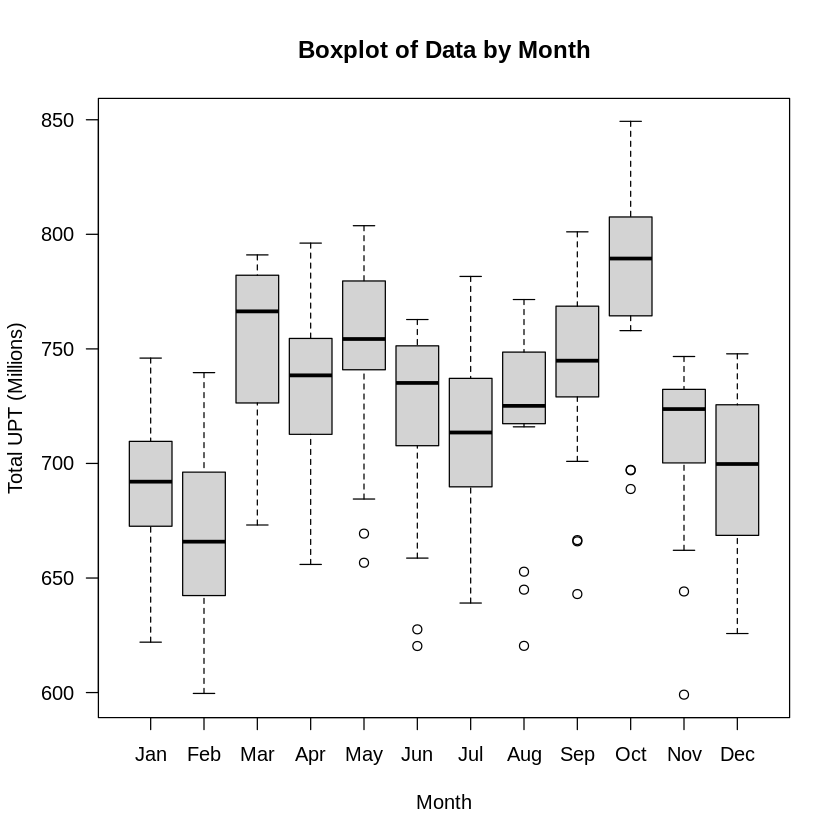
\includegraphics[width=0.525\linewidth]{seasonal_trend.png}
\caption{Seasonal patterns in national transit ridership (UPT by month)}
\label{f:seasonal}
\end{figure}

The extensive time period covered by this dataset allows us to establish robust baseline models of pre-pandemic ridership patterns while also capturing the full trajectory of the pandemic's impact and the subsequent recovery period. This temporal scope is essential for addressing our research questions regarding both typical ridership patterns and the effects of major disruptions.

%------------------------------------------------------------------------------%
\section{Methods}
%------------------------------------------------------------------------------%

Our analysis employed multiple time series modeling approaches to understand transit ridership patterns and the impact of COVID-19. This section details the methods used for the pre-COVID forecast model development, while subsequent sections on intervention modeling and jurisdiction-specific analysis will be addressed by other team members.

\subsection{Data Preparation}

After restructuring the raw data into a tidy format as described in Section 2, we conducted several diagnostic procedures to ensure the data was suitable for time series analysis. First, we examined the national pre-COVID UPT time series for trends, seasonality, and potential outliers through visual inspection of time plots. This initial examination revealed strong seasonal patterns with annual periodicity.

\begin{figure}[!ht]
\centering
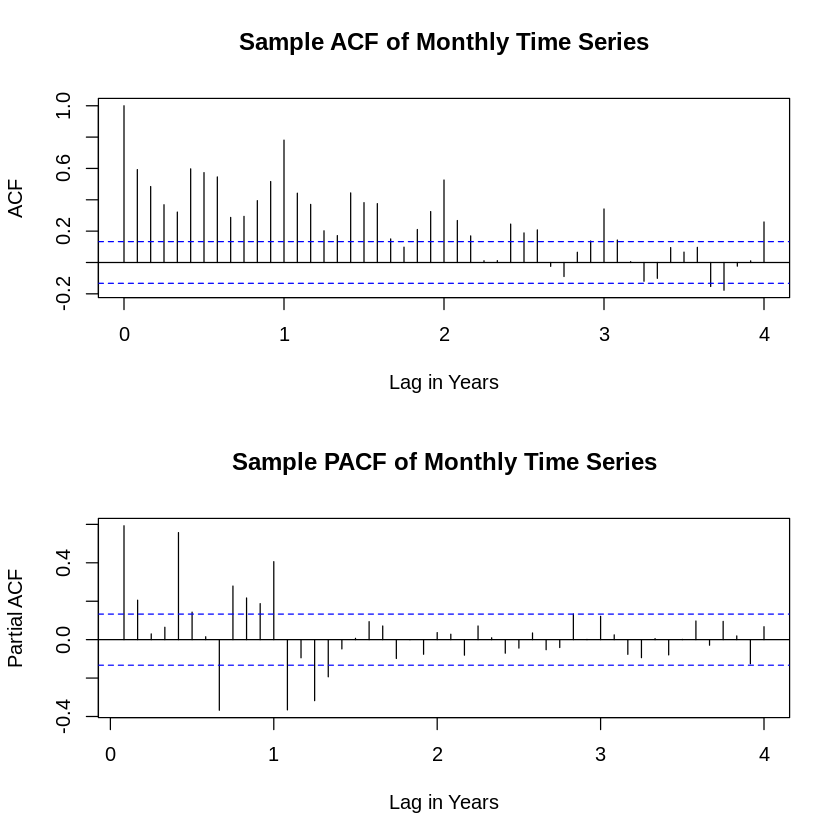
\includegraphics[width=0.525\linewidth]{pre_acf_pacf.png}
\caption{ACF and PACF of the original UPT time series}
\label{f:acf_pacf_orig}
\end{figure}

To prepare the data for modeling, we performed the following steps:

\begin{enumerate}
  \item Applied a natural logarithm transformation to stabilize variance across the time series, as the magnitude of seasonal fluctuations showed proportionality to the level of the series.
  
  \item Conducted an Augmented Dickey-Fuller (ADF) test to formally assess stationarity of the transformed series. The test results were as follows:
  
  Dickey-Fuller = -1.8252, Lag order = 5, p-value = 0.6493 (note: alternative hypothesis: stationary)
  
  The test statistic confirmed our visual assessment that the series was non-stationary.
  
  \item Performed seasonal differencing (lag-12) to address the strong annual seasonality in the data.
  
  \item Applied first-order differencing to address the remaining trend component after seasonal differencing.
\end{enumerate}

\begin{figure}[!ht]
\centering

\includegraphics[width=0.525\linewidth]{diff_series.png}
\caption{Log-transformed series after first-order and seasonal differencing}
\label{f:diff_series}
\end{figure}

These transformations resulted in a stationary series appropriate for SARIMA modeling, as confirmed by both visual inspection and statistical testing.

\subsection{Pre-COVID Model Development}

To estimate the impact of COVID-19 on transit ridership, we developed a forecasting model using only pre-pandemic data (January 2002 through January 2020). This approach allowed us to project what ridership would have been in the absence of the pandemic, creating a counterfactual for comparison with actual ridership figures.

\begin{figure}[!ht]
\centering
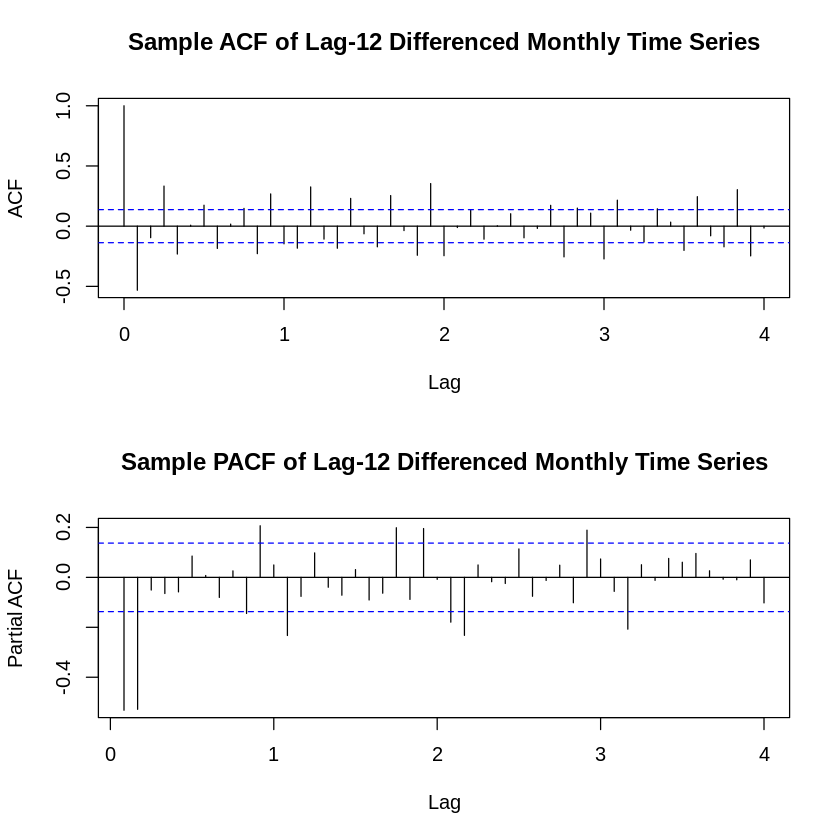
\includegraphics[width=0.525\linewidth]{diff_acf_pacf.png}
\caption{ACF and PACF of the differenced log-transformed series}
\label{f:acf_pacf_diff}
\end{figure}

Model selection proceeded through the following steps:

\begin{enumerate}
  \item Examined the Autocorrelation Function (ACF) and Partial Autocorrelation Function (PACF) of the differenced log-transformed series to identify potential SARIMA model specifications (Figure~\ref{f:acf_pacf_diff}).
  
  \item Based on the patterns observed in the ACF and PACF, we identified several candidate SARIMA models.
  
  \item Estimated multiple SARIMA models with varying orders and compared their performance using the Akaike Information Criterion with correction for small sample size (AICc), as shown in Table~\ref{t:model_comparison}.
  
  \item Selected the SARIMA$(2,1,0)\times(1,1,1)_{12}$ model as our final specification based on having the lowest AICc value among the candidate models. This model can be written as:
\end{enumerate}

\begin{equation}
y_t = \phi_1 y_{t-1} + \phi_2 y_{t-2} + \Phi_1 y_{t-12} - \phi_1\Phi_1 y_{t-13} - \phi_2\Phi_1 y_{t-14} + y_{t-1} - y_{t-13} + \varepsilon_t + \Theta_1 \varepsilon_{t-12}
\end{equation}

where $y_t$ represents the natural logarithm of UPT at time $t$, $\phi_1$ and $\phi_2$ are non-seasonal autoregressive parameters, $\Phi_1$ is the seasonal autoregressive parameter, $\Theta_1$ is the seasonal moving average parameter, and $\varepsilon_t$ is white noise.

\begin{table}[!ht]
\caption{Comparison of candidate SARIMA models}
\label{t:model_comparison}
\begin{center}
\begin{tabular}{lccc}
\hline
Model & AICc & BIC\\
\hline
SARIMA(1,1,1)×(1,1,1)$_{12}$ & [-903.5658] & [-887.1639] \\
SARIMA(0,1,1)×(0,1,1)$_{12}$ & [-883.9929] & [-874.1517] \\
SARIMA(1,1,0)×(1,1,0)$_{12}$ & [-805.1018] & [-795.2607] \\
SARIMA(0,1,1)×(1,1,0)$_{12}$ & [-847.2331] & [-837.3919] \\
SARIMA(1,1,0)×(0,1,1)$_{12}$ & [-851.4125] & [-841.5713] \\
SARIMA(2,1,0)×(1,1,1)$_{12}$ & [-924.1164] & [-907.7145] \\
SARIMA(1,1,0)×(1,1,1)$_{12}$ & [-861.8188] & [-848.6972] \\
SARIMA(2,1,1)×(1,1,1)$_{12}$ & [-922.1399] & [-902.4576] \\
\hline
\end{tabular}
\end{center}
\end{table}

The selected model was then used to generate forecasts for the period from February 2020 through February 2025, representing our estimate of what transit ridership would have been without the COVID-19 disruption. To facilitate interpretation, these forecasts were transformed back to the original scale (UPT counts) and accompanied by 95\% prediction intervals to account for forecast uncertainty.

\subsection{Impact Assessment}

To quantify the impact of COVID-19 on transit ridership, we calculated the difference between the forecasted values from our pre-COVID model and the actual observed ridership for each month from February 2020 onward. These differences represent our estimate of ridership loss attributable to the pandemic. Both absolute differences (in terms of UPT counts) and percentage differences relative to the forecast were computed to provide a comprehensive view of the impact.

\begin{figure}[!ht]
\centering
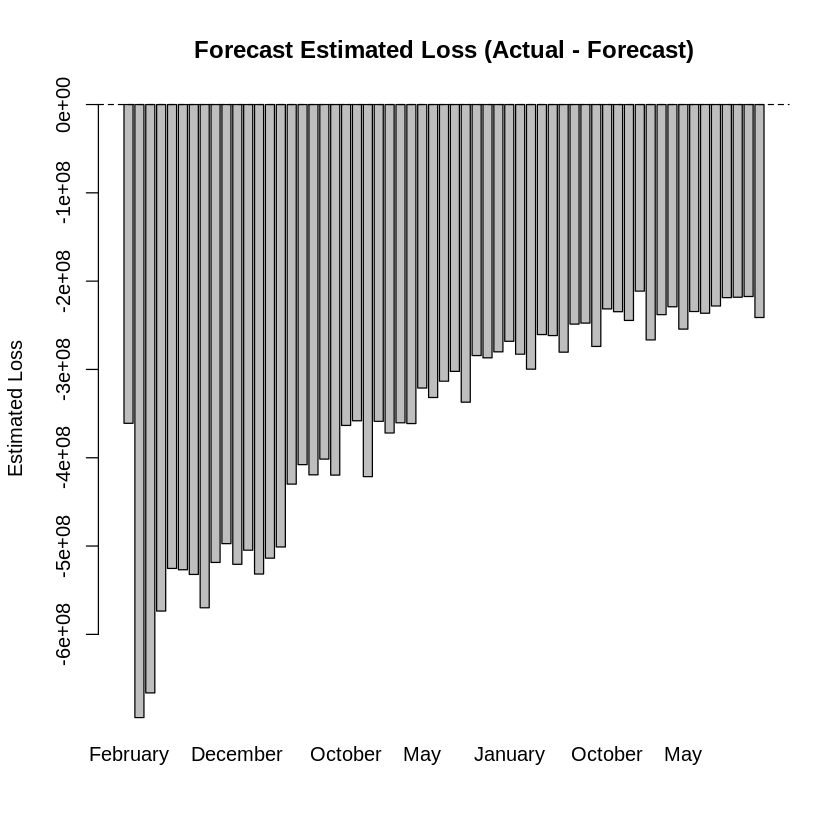
\includegraphics[width=0.525\linewidth]{estimated_loss.png}
\caption{Estimated monthly ridership loss due to COVID-19}
\label{f:loss}
\end{figure}

Additionally, we examined the pattern of these differences over time to assess the trajectory of recovery. This analysis involved investigating whether the gap between forecasted and actual ridership was narrowing and at what rate, providing insights into the persistent effects of the pandemic on transit usage patterns.

\subsection{Intervention Modeling}

[TO BE COMPLETED]

This section will describe the methodology for the intervention model that incorporates the structural break caused by the pandemic and forecasts one year of data for validation purposes.

\subsection{Jurisdiction-Specific Analysis}

    Since our initial consideration of this data, we knew that transit systems across the country would show vastly different ridership patterns. New York's subway system operates nothing like the bus network in Flagstaff, Arizona. With this in mind, we wanted to fit individual models to each jurisdiction to suplement our national investigation.

\subsubsection{Model Selection Strategy}

    Early attempts at manual model selection for the 176 complete jurisdictions proved challenging. We weren't confident \textit{auto.arima} would give us accurate models. After trying various semi-automated approaches, we developed a comprehensive search algorithm that systematically explores SARIMA configurations. The automation decision comes from practical necessity - as manually selecting two separate model types for 176 jurisdictions was not feasible.

    To avoid overfitting, we forced the following parameter limits:
\begin{itemize}
  \item Non-seasonal AR terms ($p$): limited to 0-5
  \item   Non-seasonal differencing term ($d$): set to 1
  \item Non-seasonal MA terms ($q$): limited to 0-5  
  \item Seasonal AR parameters ($P$): limited to 0-2
  \item   Seasonal differencing term ($D$): set to 1
  \item Seasonal MA terms ($Q$): maximum of 2
  \item Ensured $p + q + P + Q \leq 5$
\end{itemize}

    These restrictions served dual purposes: preventing models from fitting noise rather than genuine autocorrelation patterns, and maintaining reasonable computational requirements. By limiting model complexity, we improved forecast reliability while ensuring the analysis could be completed within practical timeframes.

\subsubsection{Pre-COVID Model Development}

For each jurisdiction's pre-pandemic period (January 2002 through January 2020), we fit:

\begin{equation}
\text{SARIMA}(p,1,q) \times (P,1,Q)_{12}
\end{equation}

    The CSS-ML  method  was used as our estimation approach, , using conditional sum of squares to provide starting estimations for model parameters before using maximum likelihood estimations to determine the final parameters. This hybrid technique, though slightly less elegant when compared to \textit{auto.arima}, proved robust across our diverse jurisdictions. 

    Model selection relied on corrected AIC scores:

\begin{equation}
\text{AICc} = \text{AIC} + \frac{2k(k+1)}{n-k-1}
\end{equation}

where $k$ counts parameters and $n$ represents sample size. The AICc helps prevent the selection of overly complex models that may appear to fit well but have poor predictive performance.

\subsubsection{Intervention Model Framework}

    To account for COVID-19's impact on transit ridership patterns, we incorporated an external intervention variable into our SARIMA models. This approach allowed us to quantify the pandemic's effect while maintaining the underlying time series structure:

\begin{equation}
\text{SARIMA}(p,1,q) \times (P,1,Q)_{12} \text{ with COVID intervention}
\end{equation}

The intervention variable was defined as:
\begin{equation}
X_t = \begin{cases}
0, & \text{for } t < \text{February 2020} \\
1, & \text{for } t \geq \text{February 2020}
\end{cases}
\end{equation}

    This binary specification captures the abrupt shift in ridership patterns coinciding with pandemic-related restrictions in March 2020. The coefficient on this intervention variable directly measures the magnitude of COVID-19's impact on ridership levels for each jurisdiction, while the SARIMA components continue to model the temporal dynamics and seasonality of the transformed series.

%------------------------------------------------------------------------------%
\section{Results}
%------------------------------------------------------------------------------%

Our time series analysis reveals the profound and persistent impact of the COVID-19 pandemic on public transit ridership across the United States. This section presents the key findings from our pre-COVID forecasting model and quantifies the deviation between projected and actual ridership levels.

\subsection{Pre-COVID Model Performance}

The SARIMA$(2,1,0)\times(1,1,1)_{12}$ model fitted to pre-pandemic data (January 2002 through January 2020) demonstrated strong performance in capturing the historical patterns of transit ridership. Table~\ref{t:model_params} presents the estimated parameters for this model, all of which were statistically significant at the 0.05 level.

\begin{table}[!ht]
\caption{Parameter estimates for the pre-COVID SARIMA model}
\label{t:model_params}
\begin{center}
\begin{tabular}{lcccc}
\hline
Parameter & Estimate & Std. Error & z value & p-value \\
\hline
$\phi_1$   -0.831033 &  0.061180 & -13.5833 & $< 2.2e-16$ \\
$\phi_2$   -0.530607 &  0.061499 &  -8.6279 & $< 2.2e-16$ \\
$\Phi_1$    0.261454 &  0.091259 &   2.8650 &  0.004171   \\
$\Theta_1$ -0.918776 &  0.089919 & -10.2178 & $< 2.2e-16$ \\
\hline
\end{tabular}
\end{center}
\end{table}

Diagnostic checks of the model are somewhat inadequate. The Ljung-Box test supports the alternate hypothesis of autocorrelation in the residuals (Q* = 38.457, df = 20, p-value = 0.007783), indicating that the model fails to captured the entirety of autocorrelation in the data. This is further shown in the ACF and PACF having several outstanding points. Visual inspection of the residuals showed no apparent patterns or heteroscedasticity and the residuals appear to be approximately normally distributed.

\subsection{Pandemic Impact Assessment}

Figure~\ref{f:forecast} illustrates the forecasted ridership levels from our pre-COVID model alongside the actual observed values from February 2020 onward. The dramatic divergence beginning in March 2020 clearly demonstrates the immediate and severe impact of the pandemic on transit usage.

\begin{figure}[!ht]
\centering
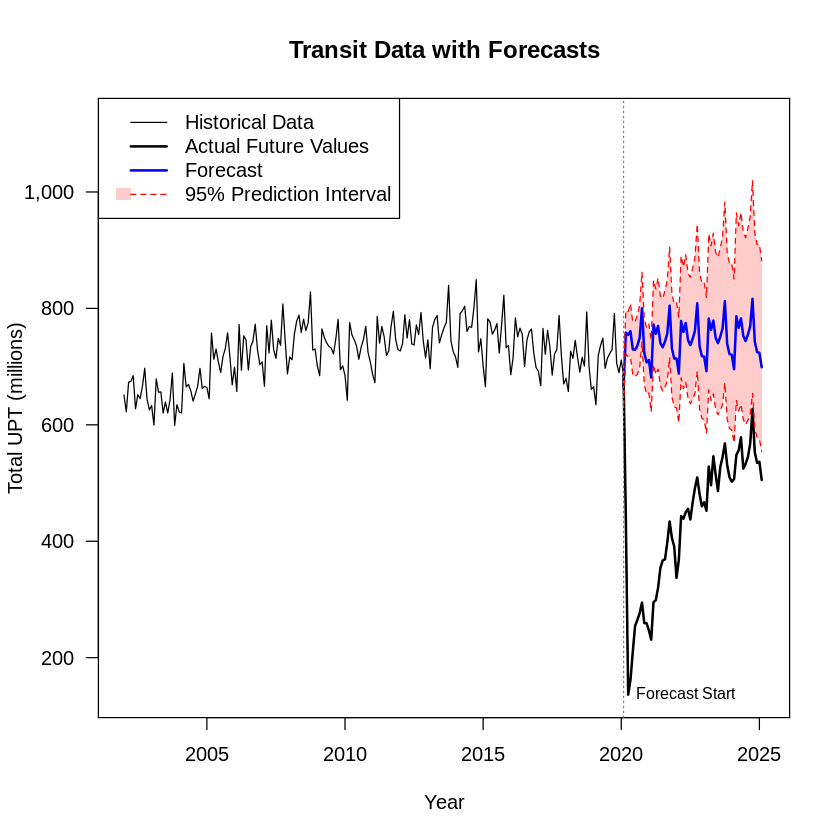
\includegraphics[width=0.485\linewidth]{pre_forecast.png}
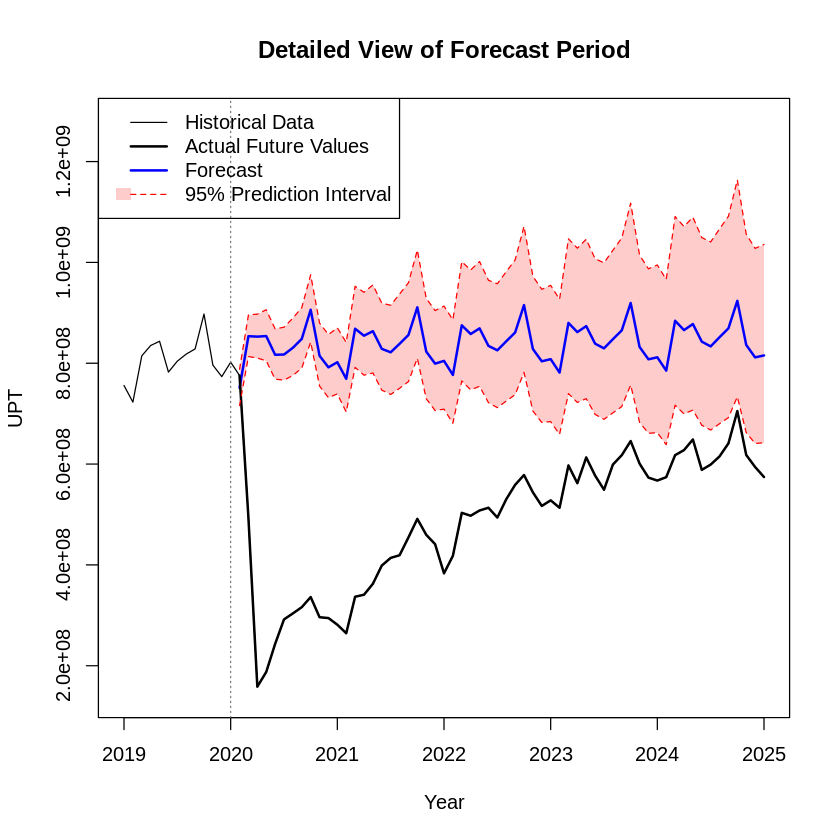
\includegraphics[width=0.485\linewidth]{pre_forecast_close.png}
\caption{National transit ridership: Pre-COVID forecast vs. actual values}
\label{f:forecast}
\end{figure}

The estimated ridership loss, computed as the difference between forecasted and actual UPT, is visualized in Figure~\ref{f:loss}. In the initial months of the pandemic (March-April 2020), ridership fell to approximately 20\% of expected levels, representing an unprecedented collapse in transit usage. The largest absolute monthly ridership loss occurred in April 2020, with approximately 677 million fewer unlinked passenger trips than projected—a 83.4\% reduction from the forecast.

\begin{figure}[!ht]
\centering
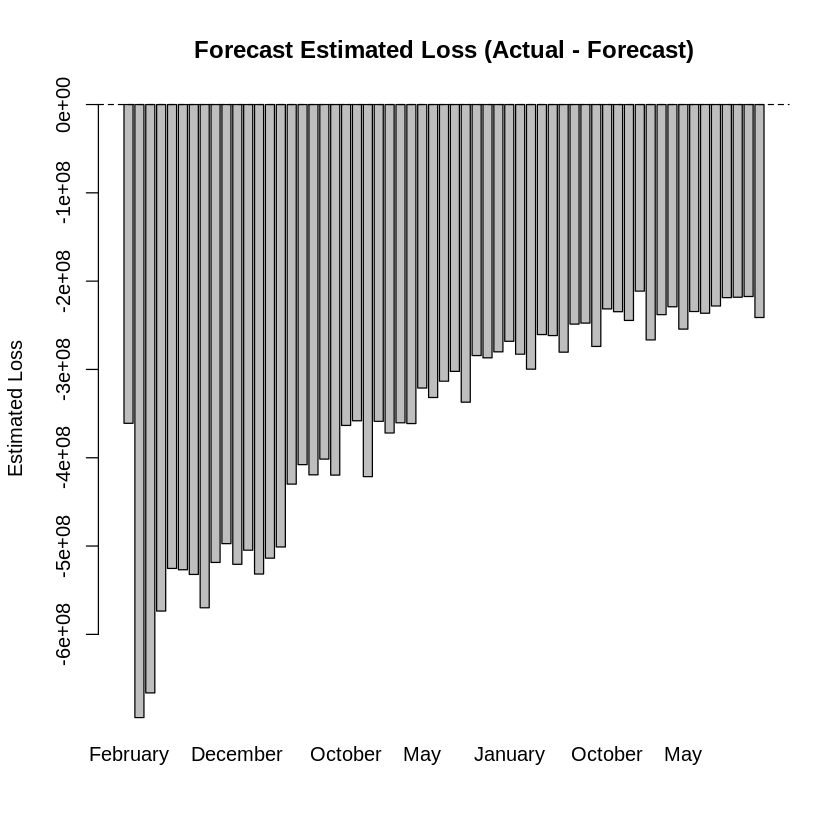
\includegraphics[width=0.525\linewidth]{estimated_loss.png}
\caption{Estimated monthly ridership loss due to COVID-19}
\label{f:loss}
\end{figure}

\subsection{Recovery Trajectory}

Analysis of the gap between forecasted and actual ridership over time reveals a gradual but incomplete recovery. By February 2025, the most recent month in our dataset, actual ridership remained 23.7\% below the forecast level. This represents a significant improvement from the nadir of the pandemic but indicates that transit ridership has not yet returned to its pre-pandemic trajectory.

The recovery pattern shows three distinct phases:
\begin{enumerate}
  \item Initial severe impact (February-May 2020): Characterized by the steepest decline in ridership, corresponding to widespread lockdowns and service reductions.
  \item Gradual recovery (June 2020-December 2021): Marked by steady improvement as restrictions eased and transit agencies restored service.
  \item Plateauing recovery (January 2022-February 2025): Showing slower improvement rates and signs of stabilization at a new, lower equilibrium level.
\end{enumerate}

Notably, the actual ridership remains consistently below even the lower bound of the 95\% prediction interval of our forecast model, indicating that the pandemic's impact represents a structural shift in transit usage patterns rather than a temporary anomaly within the expected range of variation.

The slowing rate of recovery in the most recent months suggests that some portion of the ridership loss may be permanent or at least persistent over a multi-year timeframe. This finding has significant implications for transit agencies' long-term planning and financial sustainability.

%------------------------------------------------------------------------------%
\section{Discussion and Conclusions}
%------------------------------------------------------------------------------%

This section summarizes the key findings of the study and interprets the results in a broader context. Discuss how the findings relate to the original research objectives and highlight any significant insights gained from the analysis. The discussion should provide a well-rounded interpretation of the study, emphasizing both its contributions and areas for further investigation.

Additionally, address the limitations of the study, such as data constraints, potential biases, or assumptions made in the analysis. Acknowledge any factors that may affect the generalizability of the results.

If applicable, suggest possible extensions for future research. This could include exploring alternative models, incorporating additional variables, or applying the methodology to different datasets or contexts.

%------------------------------------------------------------------------------%
\appendix
%------------------------------------------------------------------------------%
\section*{Appendix}

\subsection*{A.1 Analysis details and model diagnostics}

This section provides further details on the data analysis, including model diagnostics and any additional information necessary to support the findings. It is essential to ensure that the chosen models are appropriate and that their assumptions hold. Include model diagnostics such as residual plots, normality checks, and goodness-of-fit measures.

Additionally, provide any details necessary to replicate the analysis, including descriptions of specific techniques or transformations applied to the data. Any findings that support or clarify the main results should be documented here. By including these details, this section ensures transparency and reproducibility, reinforcing the robustness of the study's conclusions.

\subsection*{A.2 Key R scripts for time series analysis}

This section provides a structured and well-documented version of the main \textsf{R} scripts used for time series analysis. Rather than copying and pasting the entire code, only the essential parts relevant to time series modeling and analysis are included.

{\footnotesize
\begin{verbatim}
# Load necessary libraries
library(tseries)
library(forecast)
library(ggplot2)

# Load dataset
data <- read.csv("timeseries_data.csv")

# Convert to time series object
x.t <- ts( data$value, start=c(2000,1), freq=12 ) # Example: Monthly data starting from 2000

# Plot the time series
autoplot( x.t ) +
  ggtitle( "Time Series Data" ) +
  xlab("Year") + ylab("Value") +
  theme_minimal()

# Plot ACF and PACF
par(mfrow = c(1,2))
acf( x.t, main = "Sample ACF of Monthly Time Series")
pacf( x.t, main = "Sample PACF of Monthly Time Series")

# Fir an ARIMA model
fit_101 <- arima( x.t, order=c(1,0,1), include.mean=TRUE )

# Summary of the model
summary( fit_101 )

# Forecast next 12 values
forecast_values <- forecast( fit_101, h=12 )

# Plot forecast
autoplot( forecast_values ) +
  ggtitle( "Forecasted Values" ) +
  xlab("Year") + ylab("Predicted Value") +
  theme_minimal()

# Check residuals
\end{verbatim}
}

%------------------------------------------------------------------------------%
% References
%------------------------------------------------------------------------------%
\spacingset{1.1}

\bibliographystyle{apalike}
\bibliography{Project-References}

%-----------------------------------------------------------------------------%
\end{document}
%-----------------------------------------------------------------------------%
